\documentclass[12pt]{article}
\usepackage{setspace}
\doublespacing
\usepackage{caption}
\usepackage{tabularx}
\usepackage{booktabs}
\usepackage{adjustbox}
\usepackage{lipsum}
\newcolumntype{C}{>{\centering\arraybackslash}X}

% ============================================================
% METADATA
% ============================================================

\newcommand{\university}{COLUMBIA UNIVERSITY}
\newcommand{\department}{Department of Economics}

\newcommand{\classnum}{ECON UN3412}
\newcommand{\subject}{Introduction to Econometrics}
\newcommand{\semester}{Spring 2026}
\newcommand{\assignment}{Homework 6}

\newcommand{\instructors}{Seyhan Erden}
\newcommand{\instructoremail}{seyhan.erden@columbia.edu}

\newcommand{\name}{Tyler Sotomayor}
\newcommand{\email}{tyler.sotomayor@columbia.edu}

\newcommand{\duedate}{15 April 2026}

\newcommand{\sealfile}{ColumbiaSeal.png}
\newcommand{\sealsize}{0.22\textwidth}

\newcommand{\tathanksline}{Special thanks to the Teaching Assistants of \classnum}

% ============================================================
% TA LIST
% ============================================================

\newcommand{\TA}[2]{%
  {\large \textbf{#1}}\par
  \href{mailto:#2}{\texttt{#2}}\par
  \vspace{0.6cm}
}

\newcommand{\TAlist}{%
  \TA{Daniel Garcia}{dg3342@columbia.edu}
  \TA{Chris Kye}{mk4449@columbia.edu}
  \TA{Shivesh Babu Narayan}{sb5211@columbia.edu}
  \TA{Luca Salvatori}{ls4241@columbia.edu}
  \TA{Zijian Zhang}{zz3263@columbia.edu}
}

% ============================================================
% TITLE PAGE MACROS
% ============================================================

\newcommand{\maketitlepage}{%
\begin{titlepage}
\begingroup
\setlength{\parindent}{0pt}
\setlength{\parskip}{0.5em}
\centering

\vspace*{-0.8cm}
\includegraphics[width=\sealsize]{\sealfile}\par
\vspace{0.3cm}
{\LARGE \textbf{\university}}\par
{\large \department}

\vspace{1.1cm}

{\normalsize \textit{Completed in Partial Fulfillment of the Requirements of}}\par
\vspace{0.45cm}
{\Large \textbf{\classnum}}\par
{\Large \textbf{\subject}}\par
\vspace{0.3cm}
{\Large \semester}\par

\vspace{1.5cm}
{\fontfamily{lmr}\selectfont\Large\scshape \assignment}\par

\vspace{1.5cm}

{\large \textbf{\instructors}}\par
\vspace{2pt}
\href{mailto:\instructoremail}{\texttt{\instructoremail}}\par

\vspace{1.0cm}

{\large \textbf{\name}}\par
\href{mailto:\email}{\texttt{\email}}\par

\vspace*{\stretch{1}}
\endgroup
\end{titlepage}
}

\newcommand{\maketapage}{%
\begin{titlepage}
\begingroup
\setlength{\parindent}{0pt}
\setlength{\parskip}{0.45em}
\centering

{\normalsize \tathanksline}\par
\vspace{1.2cm}

\TAlist

\vspace*{\stretch{1}}
\endgroup
\end{titlepage}
}

% ------------------------------------------------------------
% LOAD TYLER'S CUSTOM MACROS AND FORMATTING
% ------------------------------------------------------------
% Import the fullpage package to adjust page margins
\usepackage{fullpage}
\usepackage{tikz}
\usepackage{pgfplots}
\pgfplotsset{compat=1.18}
\usepackage{tikz,pgfplots,caption}
\usepackage{graphicx}
\usepackage{adjustbox}
\usepackage{multicol}
\usepackage{tabularx}
\usepackage{array}
\usepackage{needspace}
\usepackage{tikz}
\usetikzlibrary{shapes,decorations,arrows,calc,arrows.meta,fit,positioning}
\newcolumntype{L}{>{\raggedright\arraybackslash}X}
\usepackage{longtable}
\usepackage{dcolumn}
\usepackage{xurl} % allows urls to break nicely across lines (recommended)

% Import the enumitem package to customize lists
\usepackage{enumitem}

% Import various AMS (American Mathematical Society) packages for mathematical symbols and formatting
\usepackage{amsfonts, amssymb, amsmath, amsthm}

% Import the mathtools package for advanced math typesetting
\usepackage{mathtools}

%For tables
\usepackage{multirow}

% Configure hyperlinks in the PDF file (e.g., author name, title)
\usepackage[pdftex, pdfauthor={\name}, pdftitle={\classnum~\assignment}]{hyperref}

% Import the xcolor package with the 'dvipsnames' option to define additional colors
\usepackage[dvipsnames]{xcolor}

% Import additional math fonts
\usepackage{bbm}

% Allow inserting images into the document
\usepackage{graphicx}

% Import additional mathematical script fonts
\usepackage{mathrsfs}

% Allow including entire PDF pages
\usepackage{pdfpages}

% Enable flexible table column formatting
\usepackage{tabularx}

% Enable landscape orientation for pages
\usepackage{pdflscape}

% Improve table formatting with multi-line cells
\usepackage{makecell}

% Improve table design and formatting
\usepackage{booktabs}

% Import natbib for better citation handling
\usepackage{natbib}

% Customize captions for tables and figures
\usepackage{caption}

% Allow subfigures within figures
\usepackage{subcaption}

% Import physics package for easier notation of derivatives, vectors, etc.
\usepackage{physics}

% Import the tcolorbox package to create colored boxes (e.g., for solutions or notes)
\usepackage[many]{tcolorbox}

% Enable conditional text inclusion (e.g., for draft versions)
\usepackage{version}

% Enable conditional logic in LaTeX (used for macros)
\usepackage{ifthen}

% Strike through mathematical expressions
\usepackage{cancel}

% Import the listings package to format source code
\usepackage{listings}

% Use the Courier font for code listings
\usepackage{courier}

% Import TikZ for creating diagrams and illustrations
\usepackage{tikz}

% Import a package for drawing game theory diagrams
\usepackage{istgame}

% Allow better placement of floating figures and tables
\usepackage{float}

% Customize hyperlink colors (e.g., blue links)
\hypersetup{
	colorlinks=true,
	linkcolor=blue,
	filecolor=magenta,
	urlcolor=blue,
}

% Adjust paragraph formatting
\setlength{\parindent}{0mm}  % No indentation at the start of paragraphs
\setlength{\parskip}{2mm}    % Space between paragraphs

% Customize numbered lists: (a), (b), (c), etc.
\setlist[enumerate]{label=({\alph*})}

% Customize nested numbered lists: (i), (ii), (iii), etc.
\setlist[enumerate, 2]{label=({\roman*})}

% Allow equations to break across pages (level 1 means minimal breaks)
\allowdisplaybreaks[1]

% Define a macro to generate a problem set header
\newcommand{\psetheader}{
	\ifthenelse{\isundefined{\collaborators}}{ % Check if collaborators are specified
		\begin{center}
			{\setlength{\parindent}{0cm} \setlength{\parskip}{0mm}
				
				% Display course number, semester, and assignment title on the left, name on the right
				{\textbf{\classnum~\semester:~\assignment} \hfill \name}
				
				% Display subject and email, with email as a clickable link
				\subject \hfill \href{mailto:\email}{\tt \email}
				
				% Display instructor names and due date
				Instructor:~\instructors \hfill Due Date:~\duedate	
				
				% Horizontal rule (separator line)
				\hrulefill}
		\end{center}
	}{
		\begin{center}
			{\setlength{\parindent}{0cm} \setlength{\parskip}{0mm}
				
				% If collaborators exist, add them as a footnote
				{\textbf{\classnum~\semester:~\assignment} \hfill \name\footnote{Collaborator(s): \collaborators}}
				
				% Display subject and email
				\subject \hfill \href{mailto:\email}{\tt \email}
				
				% Display instructor names and due date
				Instructor(s):~\instructors \hfill Due Date:~\duedate	
				
				\hrulefill}
		\end{center}
	}
}

% Customize page numbering: include class number, assignment, and page number
\usepackage{fancyhdr}
\pagestyle{fancy}
\fancyhf{}
\lfoot{\classnum~\assignment}
\rfoot{\thepage}
\renewcommand{\headrulewidth}{0pt}
\renewcommand{\footrulewidth}{0pt}

% Define a macro to format point values for problems
\makeatletter
\def\points{\@ifnextchar[{\@with}{\@without}}
\def\@with[#1]#2{{\ifthenelse{\equal{#2}{1}}{{[1 point, #1]}}{{[#2 points, #1]}}}}
\def\@without#1{\ifthenelse{\equal{#1}{1}}{{[1 point]}}{{[#1 points]}}}
\makeatother

% ---------------------------------------
% Elegant Theorem Style (Academic / Journal)
% ---------------------------------------
\newcommand{\MRS}{\operatorname{MRS}}

\makeatletter
\newtheoremstyle{econ-thm}% name
  {6pt}% Space above
  {6pt}% Space below
  {\normalfont}% Body font
  {}% Indent
  {\bfseries}% Default head font (BOLD ONLY)
  {.}% Punctuation after theorem number
  {0.5em}% Space after theorem head
  {%
    \textbf{\thmname{#1}\thmnumber{ #2}.}% <-- LABEL: bold italic
    \ifx\thmnote\@empty
    \else\ \textbf{\thmnote{#3}}\fi% <-- NAME: bold only
  }% Head spec
\makeatother

\theoremstyle{econ-thm}
\newtheorem{theorem}{Theorem}
\newtheorem{lemma}{Lemma}
\newtheorem{corollary}{Corollary}
\newtheorem{proposition}{Proposition}
\newtheorem{definition}{Definition}



% Define an environment for problems (sets text color to black)
\newenvironment{problem}[1]{\color{black} #1}{}

% Define a solution box with a green border and automatic proof environment
\newenvironment{solution}{%
  \leavevmode
  \begin{tcolorbox}[
    breakable,
    colback=green!5!white,
    colframe=green!75!black,
    enhanced jigsaw,
    % ↓ ensure no first-line indent anywhere in the box
    before upper={\parindent0pt\relax \parskip2mm}%
  ]%
  \proof[\scshape Solution:] \mbox{}\par\noindent
}{%
  \renewcommand{\qedsymbol}{$\blacksquare$}%
  \endproof
  \end{tcolorbox}%
}

% Define a reflection environment with a gray box
\newenvironment{reflection}{\begin{tcolorbox}[breakable, colback=black!8!white,colframe=black!60!white, enhanced jigsaw, parbox = false]\textsc{Reflections:}}{\end{tcolorbox}}

% Define a custom QED symbol for proofs
\newcommand{\qedh}{\renewcommand{\qedsymbol}{$\blacksquare$}\qedhere}

% Define custom colors for syntax highlighting
\definecolor{mygreen}{rgb}{0,0.6,0}
\definecolor{mygray}{rgb}{0.5,0.5,0.5}
\definecolor{mymauve}{rgb}{0.58,0,0.82}

% Define Stata programming language syntax highlighting for listings
\lstdefinelanguage{Stata}{
	% Define categories of keywords for Stata commands
	morekeywords=[1]{regress, reg, summarize, sum, display, di, generate, gen, bysort, use, import, delimited, predict, quietly, probit, margins, test},
	% Define reserved words
	morekeywords=[2]{boolean, break, byte, case, catch, class, const, continue, delete, double, else, enum, export, float, function, if, int, local, long, matrix, namespace, new, numeric, NULL, operator, pointer, private, protected, public, return, scalar, short, static, string, struct, super, switch, template, this, throw, typedef, typename, union, unsigned, using, vector, virtual, void, volatile, while,},
	% Define comment styles for Stata code
	morecomment=[l]{//},
	morecomment=[s]{/*}{*/},
	sensitive=true,
}

% Set global options for code listings (e.g., font, line numbering)
\lstset{ 
	backgroundcolor=\color{white},  
	basicstyle=\footnotesize\ttfamily, 
	numbers=left,
	numberstyle=\tiny\color{mygray},  
	keywordstyle=\color{blue},  
	commentstyle=\color{mygreen},  
	stringstyle=\color{mymauve},  
	frame=single,  
	tabsize=2,
}


% Override link colors to black
\hypersetup{citecolor=black, linkcolor=black}

\begin{document}

\pagenumbering{gobble}
\maketitlepage
\maketapage

\clearpage
\pagenumbering{roman}
\tableofcontents
\clearpage
\pagenumbering{arabic}
\psetheader

% ============================================================
% PROBLEM 1 -- AMEX CREDIT CARD APPLICANTS  (GRADED)
%   Problem statements reproduced verbatim from ps6_Spring 2026.pdf.
%   Solutions will be added in a later commit; this submission
%   focuses on the ungraded recitation exercises that were the
%   subject of Recitation 10 (SW Empirical Exercises 11.1 and 11.2).
% ============================================================

\section*{Problem 1 \points{100}}
\addcontentsline{toc}{section}{Problem 1: American Express Credit Card Applicants}

\begin{problem}
This question deals with the dataset of American Express credit card applicants \texttt{AmEx.dta}. To be able to view the dataset with STATA, you may need to write \texttt{set memory 32m} on the command window first. For each part, you will need to report results for the linear probability model, logit, and probit models. The best way to organize your results is in the form of a table. Report the log-likelihood and pseudo $R^2$ for the nonlinear models and the $R^2$ and adjusted $R^2$ for the linear model.

\smallskip
\begin{tabular}{ll}
\textit{cardhldr}:  & a binary indicator for whether or not the individual is approved as cardholder \\
\textit{income}:    & the applicant's income \\
\textit{age}:       & the applicant's age in years \\
\textit{selfempl}:  & a binary indicator for whether or not the individual is self-employed \\
\textit{ownrent}:   & an indicator for whether or not an individual owns or rents their primary residence \\
\textit{acadmos}:   & the number of months an individual has resided at their current address \\
\textit{majdrg}:    & the number of major derogatory credit events in the last 12 months \\
\textit{mindrg}:    & the number of minor derogatory credit events in the last 12 months \\
\end{tabular}
\end{problem}

\begin{enumerate}

\item
\begin{problem}{\points{3}}
First, to get the scale of the coefficients right, replace $\mathit{income} = \mathit{income}/1000$. You only need a few of the variables from the data set. So, it is a good idea to keep those and not the rest. You can do this with the following command:
\begin{verbatim}
keep cardhldr income age selfempl ownrent acadmos majordrg minordrg
\end{verbatim}
Now, what fraction of consumers in the sample are cardholders? What does this tell us in terms of external validity? (\textit{hint}: use the \texttt{tabulate} command.)
\end{problem}

\item
\begin{problem}{\points{3}}
Consider predicting whether or not an individual is approved as a cardholder \textit{cardhldr} as a function of \textit{income}, \textit{age}, \textit{selfempl}, \textit{ownrent}, \textit{acadmos}. Write commands for LPM, logit and probit.
\end{problem}

\item
\begin{problem}{\points{8}}
Compute the marginal effect (how does $\Pr(Y=1)$ change) for someone who is self-employed and for whether or not they rent or own their home. Evaluate this for an individual who has median values for their $X$ variables (covariates).
\begin{center}
\begin{tabular}{l ccc}
\toprule
                          & LPM & Logit & Probit \\ \midrule
$\Delta\mathit{selfemp}$  &     &       &        \\
$\Delta\mathit{ownrent}$  &     &       &        \\
$\%\Delta\mathit{selfemp}$ &    &       &        \\
$\%\Delta\mathit{ownrent}$ &    &       &        \\
\bottomrule
\end{tabular}
\end{center}
\end{problem}

\item
\begin{problem}{\points{15}}
Repeat the previous exercise for someone whose income is at the 20\% and 80\% of the consumers in the sample.
\end{problem}

\item
\begin{problem}{\points{5}}
Express all three cases (20\%, 50\%, 80\%) in terms of the probability ratio or log-odds. How big is the impact? Is this a lot or a little?
\end{problem}

\item
\begin{problem}{\points{4}}
Now consider a specification that includes major and minor derogatory credit events in the last year (\textit{majdrg}, \textit{mindrg}). Write commands for LPM, logit and probit.
\end{problem}

\item
\begin{problem}{\points{18}}
Report the full table of specifications (there should be 6) with all relevant statistics. Mark 1\%, 5\% and 10\% significance levels using the key at the bottom of the table.
\end{problem}

\item
\begin{problem}{\points{6}}
Which model fits the data the best? Which variables have the most explanatory power? Do major derogatory credit events matter? Do you prefer models with or without derogatory events?
\end{problem}

\item
\begin{problem}{\points{6}}
Construct a 95\% confidence interval for the effect of an additional major derogatory credit event on being an American Express cardholder under the linear probability model.
\end{problem}

\item
\begin{problem}{\points{6}}
Repeat for the logit and probit models in the case where the $x$ values take on the median values in the sample.
\end{problem}

\item
\begin{problem}{\points{8}}
Compute the fitted values for the linear probability model, and plot a histogram for the fitted values of the $y$ variable. Do the same for logit and probit models.
\end{problem}

\item
\begin{problem}{\points{6}}
What should be the domain of predicted values from the LPM? What fraction of values lies outside this domain? How do we interpret them?
\end{problem}

\item
\begin{problem}{\points{6}}
From the results you find on Table~1, what can you say about probit and logit results? How about LPM results?
\end{problem}

\item
\begin{problem}{\points{6}}
A well-known result by \citet{Amemiya1981} is that over the range of probabilities from 30\% to 70\% the following approximations should hold: $\beta_{\mathrm{LPM}} \approx 0.4\,\beta_{\mathrm{probit}}$ and $\beta_{\mathrm{LPM}} \approx 0.25\,\beta_{\mathrm{logit}}$. Take your results for logit and probit; how does this result look for $\beta_{\mathit{majordrg}}$?
\end{problem}

\end{enumerate}

\bigskip
\noindent\textit{Note.} Problem~1 above reproduces the American Express credit-card question from Problem Set 6 verbatim; solutions to parts (a)--(n) are not included in this submission. The remainder of this document solves the two recitation exercises associated with Homework~6, corresponding to Stock and Watson Empirical Exercises 11.1 and 11.2 as assigned in Recitation~10.

\newpage

% ============================================================
% RECITATION EXERCISE 1 -- SW 11.1 (UNGRADED, FULLY SOLVED)
% ============================================================

\section*{Recitation Exercise 1 \textnormal{\small (SW Empirical Exercise 11.1, ungraded)}}
\addcontentsline{toc}{section}{Recitation Exercise 1: Employment and the Great Recession (SW 11.1)}

\begin{problem}
In April 2008, the unemployment rate in the United States stood at 5.0\%. By April 2009, it had increased to 9.0\%, and it had increased further, to 10.0\% by October 2009. Were some groups of workers more likely to lose their jobs than others during the Great Recession? For example, where young workers more likely to lose their jobs than middle-aged workers? What about workers with a college degree versus those without a degree or women versus men. We will be working with \texttt{employment\_08\_09.dta}, which contains a random sample of 5,440 workers who were surveyed in April 2008 and reported that they were employed full time. The workers were surveyed one year later, in April 2009, and asked about their employment status (employed, unemployed, or out of the labor force).
\end{problem}

\begin{enumerate}

% ----- (a) -----
\item
\begin{problem}{\points{8}}
What fraction of workers in the sample were employed in April 2009? Use your answer to compute a 95\% confidence interval for the probability that a worker was employed in April 2009, conditional on being employed in April 2008.
\end{problem}
\begin{solution}
The sample consists of $n = 5{,}412$ workers who were employed full time in April 2008. The binary variable \texttt{employed} takes the value 1 if the same worker was employed (in any capacity) in April 2009 and 0 otherwise. Its sample mean is therefore the sample analogue of the conditional probability of interest, $\Pr(\text{Empl}_{09}=1 \mid \text{Empl}_{08}=1)$:
\[
\hat{p} \;=\; \frac{1}{n}\sum_{i=1}^{n} \text{employed}_i \;=\; 0.8755.
\]
Because $\text{employed}_i$ is Bernoulli, the large-sample standard error of $\hat{p}$ is
\[
\mathrm{SE}(\hat{p}) \;=\; \sqrt{\tfrac{\hat{p}(1-\hat{p})}{n}}
\;=\; \sqrt{\tfrac{0.8755 \times 0.1245}{5{,}412}} \;=\; 0.00449.
\]
Applying the standard 95\% normal approximation yields
\[
\hat{p} \pm 1.96\,\mathrm{SE}(\hat{p}) \;=\; 0.8755 \pm 0.0088 \;=\; \boxed{[\,0.8667,\; 0.8843\,]}.
\]
Roughly 86.7--88.4\% of workers employed in April 2008 were still employed one year later. The complement of this interval, $[11.6\%,13.3\%]$, gives the fraction who lost their job or left the labor force during the recessionary year. See \citet{StockWatson2020}, \S11.1, for the underlying binary-outcome setup.
\end{solution}

\begin{reflection}
The Bernoulli SE formula is a special case of the Wald standard error for a binary-response model with only an intercept: in the LPM of \texttt{employed} on a constant, the OLS coefficient equals $\hat{p}$ and the homoskedasticity-consistent SE is $\sqrt{\hat{p}(1-\hat{p})/n}$. Because the population variance of a Bernoulli equals $p(1-p)$, this SE is \emph{not} obviously biased in small samples---it is the maximum-likelihood SE---and the Wilson or exact Clopper--Pearson interval would yield only a marginally different CI here given $n=5{,}412$.

\textbf{Questions for the TA.}
\begin{enumerate}
\item[(1)] Why is $1.96$ the appropriate critical value rather than a $t$-critical value from the $t$-distribution? At what sample size does the $t$-vs-$z$ distinction matter for a Bernoulli proportion in practice?
\item[(2)] The CPS is a complex stratified sample, so ``$n=5{,}412$ independent observations'' overstates the effective sample size. How would design weights and primary-sampling-unit clustering change $\mathrm{SE}(\hat{p})$? Does the textbook ever invoke survey weights in Chapter 11 exercises, and if not, why is that considered acceptable here?
\item[(3)] When $\hat{p}$ is close to $0$ or $1$ (e.g., the unemployment rate of $0.0165$ in the 2006--2007 sample), the Wald CI can include values outside $[0,1]$. Would a Wilson or a Clopper--Pearson interval be more appropriate in that setting, and does Stata compute either by default?
\end{enumerate}
\end{reflection}

% ----- (b.i & ii) -----
\item
\begin{problem}{\points{8}}
\textbf{(b.i \& ii)} Regress \textit{Employed} on \textit{Age} and $\text{Age}^2$, using a linear probability model. Based on this regression, was age a statistically significant determinant of employment in April 2009? Is there evidence of a nonlinear effect of age on the probability of being employed?
\end{problem}
\begin{solution}
Let $E_i$ denote \texttt{employed}. The linear probability model is
\[
E_i \;=\; \beta_0 + \beta_1\,\text{age}_i + \beta_2\,\text{age}_i^2 + u_i,
\]
fit by OLS with heteroskedasticity-robust (HC1) standard errors; heteroskedasticity is inherent to the LPM because $\mathrm{Var}(E_i \mid X_i) = \Pr(E_i=1\mid X_i)\,[1-\Pr(E_i=1\mid X_i)]$ varies with $X_i$ (\citealt{StockWatson2020}, \S11.1).

The estimated equation is
\[
\boxed{\;
\widehat{\text{employed}}_i
= \underset{(0.0669)}{0.307}
+ \underset{(0.00328)}{0.0283}\,\text{age}_i
\;-\; \underset{(0.0000388)}{0.000327}\,\text{age}_i^2\;},
\]
with $n = 5{,}412$ and $R^2 = 0.0197$. Individually, $t_{\beta_1} = 8.62$ and $t_{\beta_2} = -8.42$, each with $p < 0.001$. Jointly, the robust $F$-statistic for $H_0\!:\, \beta_1 = \beta_2 = 0$ is $F(2,5409) = 37.50$ with $p < 0.001$.

\textbf{Conclusion.} Age is a statistically significant determinant of April 2009 employment at any conventional level. Because $\hat{\beta}_2$ is statistically different from zero, the relationship is \emph{nonlinear}: the quadratic specification fits better than the linear-only one. Setting $\partial \hat{E}_i/\partial \text{age} = 0$ gives a peak at age $-\hat{\beta}_1/(2\hat{\beta}_2) = 0.0283/(2 \times 0.000327) \approx 43.3$ years---the probability of still being employed in April 2009 rises from the teens to the early 40s and then declines into the 60s.
\end{solution}

% ----- (b.iii) -----
\item
\begin{problem}{\points{4}}
\textbf{(b.iii)} Using the same LPM on \textit{Age} and $\text{Age}^2$, compute the predicted probability of employment for a 20-year-old worker, a 40-year-old worker, and a 60-year-old worker.
\end{problem}
\begin{solution}
Plugging into the estimated equation (or equivalently using \texttt{margins, at(age=(20 40 60))}):
\[
\begin{array}{lccc}
\text{Age} & 20 & 40 & 60 \\
\widehat{\Pr}(\text{Empl}_{09}=1) & 0.7423 & 0.9158 & 0.8279
\end{array}
\]
These values match the inverted-U pattern identified in part (b.i\&ii): retention is lowest at the ages that bracket the peak and highest near it. Figure~\ref{fig:p1_age} plots the entire predicted age profile over $[18,63]$ for all three models.
\end{solution}

% ----- (c) Probit -----
\item
\begin{problem}{\points{6}}
\textbf{(c)} Repeat (b) using a probit regression.
\end{problem}
\begin{solution}
The probit model writes
\[
\Pr(E_i = 1 \mid X_i) = \Phi(\beta_0 + \beta_1 \text{age}_i + \beta_2 \text{age}_i^2),
\]
where $\Phi$ is the standard normal CDF. Maximum-likelihood estimation with the Huber-White sandwich variance gives
\[
\boxed{\;
\widehat{\Pr}(\text{Empl}_{09}=1)
= \Phi\!\left(\underset{(0.250)}{-1.258} + \underset{(0.0129)}{0.122}\,\text{age}_i - \underset{(0.000155)}{0.00141}\,\text{age}_i^2 \right)\;}.
\]
The pseudo-$R^2$ (McFadden) is 0.0232. Individually, $z_{\beta_1} = 9.44$ and $z_{\beta_2} = -9.09$; jointly $\chi^2(2) = 92.89$, $p < 0.001$. Age is highly significant and nonlinear. The predicted probabilities are
\[
\widehat{\Pr}(E=1 \mid \text{age}=20,40,60) = 0.7296,\; 0.9117,\; 0.8316.
\]
\end{solution}

% ----- (d) Logit -----
\item
\begin{problem}{\points{6}}
\textbf{(d)} Repeat (b) using a logit regression.
\end{problem}
\begin{solution}
The logit model replaces $\Phi$ with the logistic CDF $\Lambda(\cdot) = e^{\cdot}/(1+e^{\cdot})$:
\[
\boxed{\;
\widehat{\Pr}(\text{Empl}_{09}=1)
= \Lambda\!\left(\underset{(0.446)}{-2.490} + \underset{(0.0235)}{0.225}\,\text{age}_i - \underset{(0.000285)}{0.00262}\,\text{age}_i^2 \right)\;}.
\]
Pseudo-$R^2 = 0.0235$; $z_{\beta_1} = 9.61$, $z_{\beta_2} = -9.21$; joint $\chi^2(2) = 97.85$, $p < 0.001$. Predicted probabilities at ages $20, 40, 60$ are $0.7251$, $0.9114$, $0.8310$.

The full regression output for parts (b)--(d) is in Table~\ref{tab:prob1-bcd} in the Appendix.
\end{solution}

% ----- (e) Comparison -----
\item
\begin{problem}{\points{6}}
\textbf{(e)} Are there important differences in your answers to (b)--(d)? Explain.
\end{problem}
\begin{solution}
The three models deliver nearly identical predicted probabilities:
\[
\begin{array}{lccc}
\text{Age} & \text{LPM} & \text{Probit} & \text{Logit} \\
\hline
20 & 0.7423 & 0.7296 & 0.7251 \\
40 & 0.9158 & 0.9117 & 0.9114 \\
60 & 0.8279 & 0.8316 & 0.8310
\end{array}
\]
The maximum spread across models is about 1.7 percentage points (at age 20); at ages near the sample mean (40), the three models agree to within $\leq 0.5$ percentage points. Figure~\ref{fig:p1_age} confirms that the three predicted age profiles are virtually indistinguishable over the interior of the age distribution.

Two reasons account for this agreement. First, the sample is dominated by values of $\Pr(Y=1)$ in the $0.7$--$0.95$ range, well away from the boundaries where the LPM's linearity is most damaging. Second, over this interior range the probit and logit link functions are themselves nearly linear after appropriate rescaling---\citet{AngristPischke2009} note that $\hat{\beta}_{\mathrm{LPM}}$ is generally well-approximated by the average partial effect from probit or logit, which is precisely what this figure shows. LPM does, however, slightly overstate $\widehat{\Pr}(E=1)$ at age 20 relative to the nonlinear models, which is the familiar symptom of the LPM pulling probabilities above $1$ and below $0$ at extreme covariates.
\end{solution}

\begin{reflection}
A useful rule of thumb from \citet{CameronTrivedi2005} and \citet{Amemiya1981} is that in the interior of the probability distribution the LPM slope is approximately $0.4 \beta_{\text{probit}}$ and $0.25 \beta_{\text{logit}}$. Plugging in the \textit{age} coefficients, $0.4 \times 0.122 = 0.049$ and $0.25 \times 0.225 = 0.056$, versus the LPM's $0.0283$---larger than the rule suggests, but not wildly so given the quadratic term. The rule is most reliable when the event is common but not rare; here it is in the 88\% range, which is near the upper edge of ``interior''.

\textbf{Questions for the TA.}
\begin{enumerate}
\item[(1)] Where do the constants $0.4$ and $0.25$ come from analytically? Are they $\phi(0)$ and $\Lambda(0)(1-\Lambda(0))$ evaluated at the latent-index mean, or something else?
\item[(2)] In a quadratic specification like ours, the LPM coefficient on \textit{age} is the slope at $\text{age} = 0$, while the probit/logit ``coefficient'' has no such simple interpretation. Should we be comparing $\beta_{\mathrm{LPM}}$ to the average partial effect from probit/logit (computed via \texttt{margins, dydx(*)}) rather than to the index coefficient?
\item[(3)] In what sense does the LPM ``fail'' on the boundaries of the probability distribution? Suppose the predicted probability for some workers is $1.05$---is that a problem for inference, for prediction, or both, and what does the literature recommend (truncation, fractional logit, switching to probit, etc.)?
\end{enumerate}
\end{reflection}

% ----- (f) Full table -----
\item
\begin{problem}{\points{10}}
\textbf{(f.i \& ii)} The data set includes variables measuring the workers' educational attainment, sex, race, marital status, region of the country, and weekly earnings in April 2008. Construct a table like Table~11.2 to investigate whether the conclusions on the effect of age on employment from (b)--(d) are affected by omitted variable bias. Use the regressions in your table to discuss the characteristics of workers who were hurt most by the Great Recession.
\end{problem}
\begin{solution}
Table~\ref{tab:prob1-full} reports LPM, probit, and logit estimates for the same sample with the expanded controls. Several features stand out.

\textbf{Age and age squared.} The LPM age coefficient falls only slightly when the controls are added, from $\hat{\beta}_{\text{age}} = 0.0283$ to $0.0253$, and $\hat{\beta}_{\text{age}^2}$ from $-0.000327$ to $-0.000293$. The qualitative conclusion---that retention is an inverted-U in age, peaking in the early 40s---is therefore robust to including the full set of demographic and earnings controls. This is informative: the age profile identified in (b)--(d) was not merely reflecting composition effects along education, race, or earnings. Analogous stability holds for probit and logit.

\textbf{Workers hurt most.} Consider the LPM column, where marginal effects are directly interpretable as probability changes:
\begin{itemize}
\item \emph{Low-education workers.} Relative to advanced-degree holders, high-school dropouts had a probability of remaining employed that was $8.8$ pp lower ($p < 0.01$). Other education categories were also associated with lower retention, though not always significantly. Education is the single strongest predictor in the full model.
\item \emph{Union members.} $-5.77$ pp ($p < 0.01$). During the Great Recession, union-intensive sectors (manufacturing, construction, autos) were hardest hit; the union dummy captures this sectoral exposure even after demographics are held fixed.
\item \emph{Low earners.} Each additional \$100/week in April 2008 earnings raised retention by $0.35$ pp ($p < 0.01$). Workers at the bottom of the earnings distribution were correspondingly more vulnerable.
\item \emph{Very young and very old workers.} Predicted retention is lowest for 18--20-year-olds and falls again past age 55 (Figure~\ref{fig:p1_age}).
\item \emph{Geography.} Workers in central states were \emph{more} likely to retain employment ($+4.1$ pp, $p < 0.01$), consistent with the 2008--09 recession being concentrated in coastal finance and housing hubs.
\end{itemize}
Sex, race, and marital status have quantitatively small and mostly insignificant coefficients after controlling for the other factors, which is one piece of evidence that the Great Recession did not systematically discriminate along those lines conditional on industry/occupation composition (captured here through union status and earnings).
\end{solution}

% ----- (g) Unemployed -----
\item
\begin{problem}{\points{6}}
\textbf{(g)} The results in (a)--(f) were based on the probability of employment. Workers who are not employed can either be (i) unemployed or (ii) out the labor force. Do the conclusions you reached in (a)--(f) also hold for workers who became unemployed? (Hint: Use the binary variable \textit{Unemployed} instead of \textit{Employed}.)
\end{problem}
\begin{solution}
Switching the dependent variable to \texttt{unemployed} (which equals 1 for the 239 workers who were actively unemployed in April 2009 and 0 for both the employed and the out-of-labor-force groups) changes the sign pattern in the expected ways; see Table~\ref{tab:prob1-unemp}.

\textbf{Age.} The sign on \texttt{age} flips from positive to negative ($\hat{\beta}_{\text{age}} = -0.00506$ in the LPM) and \texttt{age}$^2$ flips from negative to positive, indicating a U-shape: young workers are most likely to \emph{become unemployed}, middle-aged workers least so, with a modest uptick toward the 60s. This mirror image of the employment profile is exactly what the labor-market flow interpretation predicts.

\textbf{Education.} High-school dropouts are a remarkable $6.99$ pp \emph{more} likely to be unemployed in April 2009 than advanced-degree holders ($p < 0.01$); high-school graduates are $3.39$ pp more likely. The monotone education gradient in employment retention from (f) becomes a sharp gradient in unemployment probability, confirming that education is the first-order determinant of recession vulnerability.

\textbf{Sex, marital status.} Women were actually \emph{less} likely to be classified as unemployed ($-2.02$ pp, $p < 0.01$)---but this is largely a labor-force attachment story, not a retention story: women who lost jobs more often exited the labor force entirely rather than actively searching. Married workers are also less likely to be unemployed conditional on losing their job.

\textbf{Union.} Curiously, the union coefficient is statistically indistinguishable from zero in the unemployment equation even though it was $-5.77$ pp in the employment equation. This is consistent with unemployed union members being more likely to eventually drop out of the labor force (or transition to early retirement) than to be captured in the April 2009 ``actively unemployed'' snapshot.

So the recession conclusions from (a)--(f) survive qualitatively---low education, young age, low earnings predict worse outcomes---but the specific demographic patterns (esp.\ women) depend crucially on which margin we study: separation vs.\ active unemployment vs.\ labor-force exit.
\end{solution}

% ----- (h) Normal times -----
\item
\begin{problem}{\points{8}}
\textbf{(h)} These results have covered employment transitions during the Great Recession, but what about transitions during normal times? On the text website, you will find the data file \textit{Employment\_06\_07}, which measures the same variables but for the years 2006--2007. Analyze these data and comment on the differences in employment transitions during recessions and normal times.
\end{problem}
\begin{solution}
In \texttt{employment\_06\_07.dta} ($n = 5{,}220$), the sample proportion of workers still employed one year later is $\hat{p}_{06} = 0.8977$ with 95\% CI $[\,0.8895, 0.9059\,]$, or approximately $2.2$ percentage points higher than the recession-era retention rate of $0.8755$. Unemployment, in turn, is only $1.65\%$ in the normal sample versus $4.42\%$ in the recession sample---a nearly three-fold increase.

Estimating the same full-controls specification on the 2006--2007 sample (Table~\ref{tab:prob1-parth}) delivers three instructive contrasts, visible in Figure~\ref{fig:p1_normal}:

\begin{enumerate}
\item \textbf{The age profile is flatter.} In normal times, predicted retention ranges from about $0.73$ at age 18 to a peak of $0.93$ near age 45 and falls to $0.83$ at age 63---a total swing of roughly $20$ pp. The 2008--2009 profile starts lower (0.68 at age 18), peaks lower ($\approx 0.915$ near age 43), and falls further ($\approx 0.79$ at age 63)---a swing of $\approx 24$ pp. The Great Recession both lowered the profile \emph{and} steepened it, hurting the young and old disproportionately.
\item \textbf{Education gradient is smaller in normal times.} High-school dropouts' retention penalty is $-5.07$ pp in normal times vs.\ $-8.82$ pp in the recession---a $75$\% amplification of the schooling gradient during the downturn. Education becomes a stronger ``moat'' during a recession.
\item \textbf{Sex effects operate differently.} Women have a larger \emph{retention} penalty in normal times ($-3.35$ pp, $p<0.01$) than in the recession ($-0.66$ pp, not significant). This is consistent with the ``he-cession'' observation that the 2008--09 downturn disproportionately struck male-dominated industries (construction, manufacturing, finance), temporarily narrowing the male--female separation gap.
\end{enumerate}

The earnings coefficient is almost identical across the two periods ($0.00357$ vs.\ $0.00348$ per \$100/week), suggesting that the earnings-to-retention pipeline is a stable feature of the labor market rather than a recession-specific phenomenon. Overall, the recession did not change \emph{who} faced higher job-loss risk; it amplified the gap between the vulnerable and the protected, particularly along the education axis.
\end{solution}

\begin{reflection}
An important caveat is that the two samples are cross-sections of different workers, so differences in estimated coefficients reflect both genuine economic changes (recession vs.\ expansion) and sampling variation. A more rigorous differences-in-differences design would interact each regressor with a recession indicator and pool the two samples---this is a natural extension but is beyond the scope of SW 11.1. The qualitative conclusions, however, are large enough to be unlikely artifacts of sampling noise.

\textbf{Questions for the TA.}
\begin{enumerate}
\item[(1)] If we pooled the 2006--07 and 2008--09 datasets and ran a single regression with a recession dummy interacted with every covariate, would the recession dummy alone identify the ``recession effect''? What identification assumption does that pooled regression require, and is it weaker or stronger than treating the two cross-sections separately?
\item[(2)] How would we test formally whether the age profile differs significantly between the two samples? A Chow test on the full vector of coefficients, or a more targeted test on $(\beta_{\text{age}}, \beta_{\text{age}^2})$? Are the cluster-robust SEs we'd want for that test the same as the heteroskedasticity-robust SEs we have here?
\item[(3)] The CPS rotates households into the sample for 4 months on, 8 months off, then 4 months on. Is it possible that some workers appear in \emph{both} the 2006--07 and 2008--09 panels? If so, how would that biased the comparison, and how could we check or correct for it?
\end{enumerate}
\end{reflection}

\end{enumerate}

\newpage

% ============================================================
% RECITATION EXERCISE 2 -- SW 11.2 (UNGRADED, FULLY SOLVED)
% ============================================================

\section*{Recitation Exercise 2 \textnormal{\small (SW Empirical Exercise 11.2, ungraded)}}
\addcontentsline{toc}{section}{Recitation Exercise 2: Workplace Smoking Bans (SW 11.2)}

\begin{problem}
Workers used to be able to smoke inside office buildings (now some students vape inside classrooms). Smoking bans were introduced in several office areas during the 1990s. Supporters of these bans argued that in addition to eliminating the externality of secondhand smoke, they would encourage smokers to quit by reducing their opportunities to smoke. We will use \texttt{smoking.dta}, which has data on 10,000 U.S.\ indoor workers from 1991 to 1993. The data set contains information on whether individuals were subject to a workplace smoking ban, whether the individuals themselves smoked, and other characteristics.
\end{problem}

\begin{enumerate}

% ----- (a) -----
\item
\begin{problem}{\points{8}}
Estimate the probability of smoking for (i) all workers, (ii) workers affected by workplace smoking bans, and (iii) workers not affected by workplace smoking bans.
\end{problem}
\begin{solution}
The sample analogues of these three conditional probabilities are the corresponding sample means of the binary variable \texttt{smoker}:
\[
\begin{array}{lccc}
\text{Group} & \hat{p} & \mathrm{SE}(\hat{p}) & n \\
\hline
\text{All workers} & 0.2423 & 0.0043 & 10{,}000 \\
\text{Workers with a workplace ban} \;(\texttt{smkban}=1) & 0.2120 & 0.0052 & 6{,}098 \\
\text{Workers without a workplace ban} \;(\texttt{smkban}=0) & 0.2896 & 0.0073 & 3{,}902
\end{array}
\]
The standard errors are the Bernoulli formula applied within each cell. The raw difference in smoking rates is $\hat{p}_{\text{no ban}} - \hat{p}_{\text{ban}} = 0.2896 - 0.2120 = 0.0776$, or about a $7.8$-percentage-point higher smoking rate among workers not covered by a ban. The key causal question---whether this difference reflects the ban's effect or pre-existing selection of smokers into non-ban workplaces---is addressed in part (c).
\end{solution}

% ----- (b) -----
\item
\begin{problem}{\points{8}}
What is the difference in the probability of smoking between workers affected by a workplace smoking ban and workers not affected by a workplace smoking ban? Use a linear probability model to determine whether this difference is statistically significant.
\end{problem}
\begin{solution}
Regressing \texttt{smoker} on \texttt{smkban} alone yields
\[
\boxed{\;
\widehat{\Pr}(\text{smoker}=1)
= \underset{(0.00726)}{0.290}
\;-\; \underset{(0.00895)}{0.0776}\,\texttt{smkban}\;},
\]
$n = 10{,}000$, $R^2 = 0.0078$. Because \texttt{smkban} is the only regressor, the slope coefficient coincides with the raw difference in means from part (a): $\hat{\beta}_{\texttt{smkban}} = -0.0776$, and the intercept equals the cell mean for non-ban workers ($0.2896$). The robust $t$-statistic is $t = -0.0776/0.00895 = -8.67$ (equivalently, $F(1, 9998) = 75.06$, $p < 0.0001$), which rejects $H_0\!:\,\beta_{\texttt{smkban}} = 0$ at any conventional significance level. The $95\%$ CI is $[\,-0.095, -0.060\,]$.

\textbf{Interpretation (cautionary).} The unconditional $7.8$-pp gap cannot be read as the causal effect of a ban. Workplaces that adopted bans in the early 1990s were more likely to be in office sectors with higher-education workforces, where smoking was already less prevalent. Part (c) repeats the exercise with controls to assess how much of the raw gap is attributable to such composition effects.
\end{solution}

% ----- (c) -----
\item
\begin{problem}{\points{8}}
Estimate a linear probability model with \textit{smoker} as the dependent variable and the following regressors: \textit{smkban}, \textit{female}, \textit{age}, $\text{age}^2$, \textit{hsdrop}, \textit{hsgrad}, \textit{colsome}, \textit{colgrad}, \textit{black}, and \textit{hispanic}. Compare the estimated effect of a smoking ban from this regression with your answer from (b). Suggest an explanation, based on the substance of this regression, for the change in the estimated effect of a smoking ban between (b) and (c).
\end{problem}
\begin{solution}
Table~\ref{tab:prob2-lpm} reports both the simple LPM from (b) and the full-controls LPM. Holding demographic and education characteristics fixed, the coefficient on \texttt{smkban} falls (in absolute value) from $-0.0776$ to
\[
\hat{\beta}_{\texttt{smkban}}^{\mathrm{full}} = -0.0472 \qquad (\mathrm{SE} = 0.0090),
\]
a reduction of approximately $40\%$. The included controls absorb a large share of the raw gap through two substantive channels:

\begin{enumerate}
\item \textbf{Education.} The education coefficients are large and monotone: relative to advanced-degree workers, smoking probability rises by $4.5$ pp for college grads, $16.4$ pp for some-college, $23.3$ pp for high-school grads, and $32.3$ pp for high-school dropouts (all $p < 0.01$). The sample correlation between \texttt{smkban} and education is positive---bans were most common in high-education workplaces---so failing to condition on education in part (b) biased $\hat{\beta}_{\texttt{smkban}}$ downward (more negative).
\item \textbf{Demographics.} Smoking probability is $3.3$ pp lower for women, $2.8$ pp lower for Black workers, and $10.5$ pp lower for Hispanic workers; it is modestly hump-shaped in age. These factors are also correlated with \texttt{smkban} coverage, contributing to the attenuation.
\end{enumerate}

\textbf{Conclusion.} Of the raw $7.8$-pp gap in part (b), about $3.0$ pp was composition (selection into ban-covered workplaces), leaving a conditional ban effect of $4.7$ pp. Under a conditional-independence assumption (the ban is ``as good as random'' given observed covariates), this $-4.7$ pp estimate is a credible causal effect.
\end{solution}

% ----- (d) -----
\item
\begin{problem}{\points{5}}
Test the hypothesis that the coefficient on \textit{smkban} is 0 in the population version of the regression in (c) against the alternative that it is nonzero, at the 5\% significance level.
\end{problem}
\begin{solution}
The test statistic is the robust $F$-statistic $F(1,9989) = 27.76$ with $p < 0.0001$ (equivalently, $t = -\sqrt{27.76} = -5.27$). Because $27.76 \gg F_{0.05}(1,\infty) = 3.84$, we reject $H_0\!:\,\beta_{\texttt{smkban}} = 0$ at the 5\% level (and at any conventional level). The estimated ban effect of $-4.7$ pp is statistically distinguishable from zero with very high confidence.
\end{solution}

% ----- (e) -----
\item
\begin{problem}{\points{6}}
Test the hypothesis that the probability of smoking does not depend on the level of education in the regression in (c). Does the probability of smoking increase or decrease with the level of education?
\end{problem}
\begin{solution}
The null hypothesis is $H_0\!:\,\beta_{\texttt{hsdrop}} = \beta_{\texttt{hsgrad}} = \beta_{\texttt{colsome}} = \beta_{\texttt{colgrad}} = 0$. The robust $F$-statistic is
\[
F(4, 9989) = 140.09, \qquad p < 0.0001,
\]
so we decisively reject. Education matters. Examining the individual coefficients,
\[
\hat{\beta}_{\texttt{hsdrop}} = 0.323 \;>\; \hat{\beta}_{\texttt{hsgrad}} = 0.233 \;>\; \hat{\beta}_{\texttt{colsome}} = 0.164 \;>\; \hat{\beta}_{\texttt{colgrad}} = 0.0448 \;>\; 0 \;(\texttt{advanced, omitted}),
\]
with all four coefficients significant at the 1\% level. The probability of smoking \emph{decreases monotonically with the level of education}: a high-school dropout is $28$ pp more likely to smoke than a college graduate and $32$ pp more likely than an advanced-degree holder, holding all other covariates fixed. Figure~\ref{fig:p2_educ} visualizes this gradient.
\end{solution}

\begin{reflection}
Although the point of SW 11.2 is to illustrate hypothesis testing in binary-response models, the substantive conclusion---strong education gradient in smoking---echoes the wider public-health literature. \citet{Evans1999} document similar patterns and estimate comparable workplace-ban effects ($3$--$5$ pp) using alternative empirical designs. The $R^2$ of the full model ($0.057$) is modest: education and demographics explain only a small fraction of who smokes, reflecting the importance of unmodeled factors like family history, peer effects, and local tobacco prices.

\textbf{Questions for the TA.}
\begin{enumerate}
\item[(1)] In the joint $F$-test for the four education dummies, the within-test SEs are still heteroskedasticity-robust. Is the standard $F$-statistic still asymptotically chi-squared under heteroskedasticity, or do we need a Wald-type test based on the robust variance matrix? Stata's \texttt{test} command after \texttt{reg, robust} appears to use the robust matrix automatically---can we confirm that?
\item[(2)] We rejected $H_0$ for both the joint education test and the individual \texttt{smkban} test. How concerned should we be about multiple testing here, given that this is one of many hypotheses we could form on the same regression? Would a Bonferroni or Holm correction change any of our conclusions at the 5\% level?
\item[(3)] The conditional-independence assumption underlying the $-4.7$ pp causal interpretation requires that, conditional on demographics and education, ban coverage is ``as good as random''. What's a plausible violation of that assumption, and what kind of natural-experiment design (state-level ban variation, employer policy changes, etc.) would help us address it?
\end{enumerate}
\end{reflection}

% ----- (f) Probit -----
\item
\begin{problem}{\points{9}}
Repeat (c)--(e) using a probit model.
\end{problem}
\begin{solution}
Table~\ref{tab:prob2-vs} presents the probit estimates alongside the LPM. All coefficients retain their signs and their relative magnitudes follow the LPM ordering, but the probit coefficients are on the latent-index (z-score) scale and not directly interpretable as probability changes.

\textbf{(c)-analogue: magnitude of the ban effect.} The probit index coefficient on \texttt{smkban} is $-0.159$ (robust SE $0.0291$). Converting to an average partial effect (APE) via \texttt{margins, dydx(smkban)}:
\[
\overline{\widehat{\partial \Pr(\text{smoker})/\partial \texttt{smkban}}} = -0.0468 \;(\mathrm{SE}=0.0086),
\]
which is essentially identical to the LPM estimate of $-0.0472$. Because the probability of smoking in this sample is in the $0.10$--$0.43$ range---well inside the ``interior'' where probit and LPM agree (\citealt{AngristPischke2009}, Ch.~3)---the two models produce indistinguishable average partial effects.

\textbf{(d)-analogue: significance of \texttt{smkban}.} The Wald $\chi^2(1) = 29.70$ ($p < 0.0001$) rejects $H_0\!:\,\beta_{\texttt{smkban}} = 0$ at any conventional significance level, mirroring the LPM conclusion.

\textbf{(e)-analogue: joint significance of education.} The joint Wald $\chi^2(4) = 447.34$ ($p < 0.0001$) again rejects the null that the four education dummies are jointly zero. The monotone pattern is identical to the LPM: smoking probability falls sharply as education rises.

\textbf{Summary.} The probit does not overturn a single substantive conclusion from (c)--(e). The qualitative takeaways (ban reduces smoking by $\approx 5$ pp; education is the strongest predictor; smoking falls monotonically with education) are identical across models. This is a useful illustration of \citet{Amemiya1981}'s result that LPM and nonlinear latent-variable models typically deliver very similar average partial effects in the interior of the probability distribution---which is why many applied economists (e.g., \citealt{AngristPischke2009}) prefer the LPM's computational simplicity and robust-SE interpretation unless the outcome is very rare or very common.
\end{solution}

\end{enumerate}

\newpage

% ============================================================
% APPENDIX
% ============================================================

\appendix
\section*{Appendix: Tables and Figures}
\addcontentsline{toc}{section}{Appendix: Tables and Figures}

\subsection*{Tables}
\singlespacing

\begin{table}[H]\centering\small
\def\sym#1{\ifmmode^{#1}\else\(^{#1}\)\fi}
\caption{Effect of Age on the Probability of Employment in April 2009\label{tab:prob1-bcd}}
\begin{tabular}{l*{3}{c}}
\toprule
                    &\multicolumn{1}{c}{(1)}&\multicolumn{1}{c}{(2)}&\multicolumn{1}{c}{(3)}\\
                    &\multicolumn{1}{c}{LPM}&\multicolumn{1}{c}{Probit}&\multicolumn{1}{c}{Logit}\\
\midrule
main                &                     &                     &                     \\
Age                 &      0.0283\sym{***}&       0.122\sym{***}&       0.225\sym{***}\\
                    &   (0.00328)         &    (0.0129)         &    (0.0235)         \\
\addlinespace
age squared         &   -0.000327\sym{***}&    -0.00141\sym{***}&    -0.00262\sym{***}\\
                    & (0.0000388)         &  (0.000155)         &  (0.000285)         \\
\addlinespace
Constant            &       0.307\sym{***}&      -1.258\sym{***}&      -2.490\sym{***}\\
                    &    (0.0669)         &     (0.250)         &     (0.446)         \\
\midrule
Observations        &       5,412         &       5,412         &       5,412         \\
$R^2$               &      0.0197         &                     &                     \\
Pseudo $R^2$        &                     &      0.0232         &      0.0235         \\
Log-likelihood      &    -1628.68         &    -1986.92         &    -1986.43         \\
\bottomrule
\multicolumn{4}{l}{\footnotesize Standard errors in parentheses}\\
\multicolumn{4}{l}{\footnotesize Heteroskedasticity-robust standard errors in parentheses.}\\
\multicolumn{4}{l}{\footnotesize Dependent variable = 1 if employed in April 2009, conditional on employment in April 2008.}\\
\multicolumn{4}{l}{\footnotesize \sym{*} \(p<0.10\), \sym{**} \(p<0.05\), \sym{***} \(p<0.01\)}\\
\end{tabular}
\end{table}


\clearpage
\begin{table}[htbp]\centering
\def\sym#1{\ifmmode^{#1}\else\(^{#1}\)\fi}
\caption{Determinants of Employment Retention, April 2008 to April 2009\label{tab:prob1-full}}
\begin{tabular}{l*{3}{c}}
\toprule
                    &\multicolumn{1}{c}{(1)}&\multicolumn{1}{c}{(2)}&\multicolumn{1}{c}{(3)}\\
                    &\multicolumn{1}{c}{LPM}&\multicolumn{1}{c}{Probit}&\multicolumn{1}{c}{Logit}\\
\midrule
main                &                     &                     &                     \\
Age                 &      0.0253\sym{***}&       0.108\sym{***}&       0.197\sym{***}\\
                    &   (0.00355)         &    (0.0147)         &    (0.0272)         \\
\addlinespace
age squared         &   -0.000293\sym{***}&    -0.00127\sym{***}&    -0.00231\sym{***}\\
                    & (0.0000419)         &  (0.000176)         &  (0.000327)         \\
\addlinespace
female              &    -0.00664         &     -0.0349         &     -0.0530         \\
                    &    (0.0100)         &    (0.0502)         &    (0.0942)         \\
\addlinespace
=1 if race != white &     -0.0186         &     -0.0814         &      -0.146         \\
                    &    (0.0138)         &    (0.0632)         &     (0.117)         \\
\addlinespace
married             &    -0.00191         &    -0.00954         &     -0.0314         \\
                    &    (0.0104)         &    (0.0532)         &     (0.101)         \\
\addlinespace
union               &     -0.0577\sym{***}&      -0.291\sym{***}&      -0.533\sym{***}\\
                    &    (0.0149)         &    (0.0650)         &     (0.119)         \\
\addlinespace
ne\_states           &      0.0164         &      0.0917         &       0.154         \\
                    &    (0.0143)         &    (0.0689)         &     (0.128)         \\
\addlinespace
so\_states           &      0.0151         &      0.0719         &       0.134         \\
                    &    (0.0135)         &    (0.0641)         &     (0.119)         \\
\addlinespace
ce\_states           &      0.0406\sym{***}&       0.209\sym{***}&       0.395\sym{***}\\
                    &    (0.0134)         &    (0.0687)         &     (0.130)         \\
\addlinespace
educ\_lths           &     -0.0882\sym{***}&      -0.373\sym{***}&      -0.637\sym{***}\\
                    &    (0.0268)         &     (0.118)         &     (0.221)         \\
\addlinespace
educ\_hs             &     -0.0251         &      -0.136         &      -0.233         \\
                    &    (0.0164)         &    (0.0924)         &     (0.179)         \\
\addlinespace
educ\_somecol        &    -0.00509         &     -0.0361         &     -0.0542         \\
                    &    (0.0167)         &    (0.0970)         &     (0.189)         \\
\addlinespace
educ\_aa             &     0.00316         &      0.0122         &      0.0379         \\
                    &    (0.0179)         &     (0.109)         &     (0.213)         \\
\addlinespace
educ\_bac            &     -0.0162         &     -0.0976         &      -0.179         \\
                    &    (0.0152)         &    (0.0918)         &     (0.178)         \\
\addlinespace
Weekly earnings, Apr. 2008 (per 100 USD)&     0.00348\sym{***}&      0.0217\sym{***}&      0.0444\sym{***}\\
                    &  (0.000953)         &   (0.00600)         &    (0.0125)         \\
\addlinespace
Constant            &       0.356\sym{***}&      -1.047\sym{***}&      -2.063\sym{***}\\
                    &    (0.0716)         &     (0.288)         &     (0.524)         \\
\midrule
Observations        &       4,773         &       4,773         &       4,773         \\
$R^2$               &      0.0355         &                     &                     \\
Pseudo $R^2$        &                     &      0.0451         &      0.0450         \\
Log-likelihood      &    -1402.86         &    -1716.01         &    -1716.18         \\
\bottomrule
\multicolumn{4}{l}{\footnotesize Standard errors in parentheses}\\
\multicolumn{4}{l}{\footnotesize Heteroskedasticity-robust standard errors in parentheses.}\\
\multicolumn{4}{l}{\footnotesize Omitted reference groups: white, western region, advanced degree.}\\
\multicolumn{4}{l}{\footnotesize \sym{*} \(p<0.10\), \sym{**} \(p<0.05\), \sym{***} \(p<0.01\)}\\
\end{tabular}
\end{table}


\clearpage
\begin{table}[htbp]\centering
\def\sym#1{\ifmmode^{#1}\else\(^{#1}\)\fi}
\caption{Determinants of Becoming Unemployed by April 2009\label{tab:prob1-unemp}}
\begin{tabular}{l*{3}{c}}
\toprule
                    &\multicolumn{1}{c}{(1)}&\multicolumn{1}{c}{(2)}&\multicolumn{1}{c}{(3)}\\
                    &\multicolumn{1}{c}{LPM}&\multicolumn{1}{c}{Probit}&\multicolumn{1}{c}{Logit}\\
\midrule
main                &                     &                     &                     \\
Age                 &    -0.00506\sym{**} &     -0.0438\sym{**} &     -0.0898\sym{**} \\
                    &   (0.00232)         &    (0.0195)         &    (0.0415)         \\
\addlinespace
age squared         &   0.0000601\sym{**} &    0.000537\sym{**} &     0.00110\sym{**} \\
                    & (0.0000271)         &  (0.000234)         &  (0.000499)         \\
\addlinespace
female              &     -0.0202\sym{***}&      -0.209\sym{***}&      -0.452\sym{***}\\
                    &   (0.00662)         &    (0.0666)         &     (0.145)         \\
\addlinespace
=1 if race != white &     0.00983         &       0.104         &       0.192         \\
                    &   (0.00934)         &    (0.0837)         &     (0.179)         \\
\addlinespace
married             &     -0.0151\sym{**} &      -0.159\sym{**} &      -0.327\sym{**} \\
                    &   (0.00726)         &    (0.0705)         &     (0.155)         \\
\addlinespace
union               &     0.00119         &    -0.00468         &      0.0160         \\
                    &   (0.00875)         &    (0.0916)         &     (0.200)         \\
\addlinespace
ne\_states           &     -0.0182\sym{**} &      -0.175\sym{*}  &      -0.401\sym{*}  \\
                    &   (0.00922)         &    (0.0946)         &     (0.206)         \\
\addlinespace
so\_states           &    -0.00974         &     -0.0796         &      -0.192         \\
                    &   (0.00904)         &    (0.0836)         &     (0.178)         \\
\addlinespace
ce\_states           &     -0.0143         &      -0.130         &      -0.306         \\
                    &   (0.00909)         &    (0.0887)         &     (0.194)         \\
\addlinespace
educ\_lths           &      0.0699\sym{***}&       0.627\sym{***}&       1.347\sym{***}\\
                    &    (0.0189)         &     (0.161)         &     (0.361)         \\
\addlinespace
educ\_hs             &      0.0339\sym{***}&       0.397\sym{***}&       0.892\sym{***}\\
                    &    (0.0100)         &     (0.134)         &     (0.314)         \\
\addlinespace
educ\_somecol        &      0.0112         &       0.186         &       0.443         \\
                    &    (0.0101)         &     (0.143)         &     (0.337)         \\
\addlinespace
educ\_aa             &     0.00936         &       0.145         &       0.338         \\
                    &    (0.0105)         &     (0.158)         &     (0.370)         \\
\addlinespace
educ\_bac            &      0.0124         &       0.193         &       0.440         \\
                    &   (0.00897)         &     (0.137)         &     (0.323)         \\
\addlinespace
Weekly earnings, Apr. 2008 (per 100 USD)&   -0.000378         &    -0.00433         &    -0.00892         \\
                    &  (0.000645)         &   (0.00738)         &    (0.0170)         \\
\addlinespace
Constant            &       0.158\sym{***}&      -0.823\sym{**} &      -1.295         \\
                    &    (0.0457)         &     (0.381)         &     (0.803)         \\
\midrule
Observations        &       4,773         &       4,773         &       4,773         \\
$R^2$               &      0.0154         &                     &                     \\
Pseudo $R^2$        &                     &      0.0371         &      0.0369         \\
Log-likelihood      &      619.68         &     -887.65         &     -887.83         \\
\bottomrule
\multicolumn{4}{l}{\footnotesize Standard errors in parentheses}\\
\multicolumn{4}{l}{\footnotesize Heteroskedasticity-robust standard errors in parentheses.}\\
\multicolumn{4}{l}{\footnotesize Dependent variable = 1 if unemployed in April 2009; =0 otherwise (including out-of-labor-force).}\\
\multicolumn{4}{l}{\footnotesize \sym{*} \(p<0.10\), \sym{**} \(p<0.05\), \sym{***} \(p<0.01\)}\\
\end{tabular}
\end{table}


\clearpage
\begin{table}[H]\centering\footnotesize\renewcommand{\arraystretch}{0.92}
\def\sym#1{\ifmmode^{#1}\else\(^{#1}\)\fi}
\caption{Determinants of Employment Retention, April 2006 to April 2007 (Normal Times)\label{tab:prob1-parth}}
\begin{tabular}{l*{3}{c}}
\toprule
                    &\multicolumn{1}{c}{(1)}&\multicolumn{1}{c}{(2)}&\multicolumn{1}{c}{(3)}\\
                    &\multicolumn{1}{c}{LPM}&\multicolumn{1}{c}{Probit}&\multicolumn{1}{c}{Logit}\\
\midrule
main                &                     &                     &                     \\
Age                 &      0.0198\sym{***}&      0.0908\sym{***}&       0.166\sym{***}\\
                    &   (0.00341)         &    (0.0158)         &    (0.0300)         \\
\addlinespace
age squared         &   -0.000230\sym{***}&    -0.00108\sym{***}&    -0.00196\sym{***}\\
                    & (0.0000403)         &  (0.000191)         &  (0.000365)         \\
\addlinespace
female              &     -0.0335\sym{***}&      -0.196\sym{***}&      -0.366\sym{***}\\
                    &   (0.00916)         &    (0.0544)         &     (0.106)         \\
\addlinespace
=1 if race != white &     -0.0154         &     -0.0707         &      -0.143         \\
                    &    (0.0133)         &    (0.0713)         &     (0.136)         \\
\addlinespace
married             &      0.0225\sym{**} &       0.139\sym{**} &       0.250\sym{**} \\
                    &   (0.00990)         &    (0.0567)         &     (0.111)         \\
\addlinespace
union               &     -0.0119         &      -0.103         &      -0.188         \\
                    &    (0.0132)         &    (0.0800)         &     (0.156)         \\
\addlinespace
ne\_states           &     0.00125         &      0.0161         &      0.0291         \\
                    &    (0.0136)         &    (0.0786)         &     (0.152)         \\
\addlinespace
so\_states           &     0.00620         &      0.0414         &      0.0675         \\
                    &    (0.0125)         &    (0.0719)         &     (0.139)         \\
\addlinespace
ce\_states           &      0.0182         &       0.109         &       0.218         \\
                    &    (0.0125)         &    (0.0743)         &     (0.144)         \\
\addlinespace
educ\_lths           &     -0.0507\sym{**} &      -0.208         &      -0.376         \\
                    &    (0.0239)         &     (0.131)         &     (0.254)         \\
\addlinespace
educ\_hs             &    -0.00802         &     -0.0362         &     -0.0532         \\
                    &    (0.0153)         &     (0.108)         &     (0.218)         \\
\addlinespace
educ\_somecol        &    -0.00104         &    0.000465         &      0.0312         \\
                    &    (0.0164)         &     (0.115)         &     (0.230)         \\
\addlinespace
educ\_aa             &      0.0118         &      0.0735         &       0.161         \\
                    &    (0.0171)         &     (0.125)         &     (0.252)         \\
\addlinespace
educ\_bac            &     0.00140         &     0.00412         &      0.0142         \\
                    &    (0.0143)         &     (0.110)         &     (0.223)         \\
\addlinespace
Weekly earnings, Apr. 2006 (per 100 USD)&     0.00357\sym{***}&      0.0305\sym{***}&      0.0675\sym{***}\\
                    &  (0.000824)         &   (0.00742)         &    (0.0164)         \\
\addlinespace
Constant            &       0.481\sym{***}&      -0.661\sym{**} &      -1.404\sym{**} \\
                    &    (0.0686)         &     (0.309)         &     (0.580)         \\
\midrule
Observations        &       4,569         &       4,569         &       4,569         \\
$R^2$               &      0.0359         &                     &                     \\
Pseudo $R^2$        &                     &      0.0535         &      0.0542         \\
Log-likelihood      &     -903.55         &    -1408.07         &    -1407.05         \\
\bottomrule
\multicolumn{4}{l}{\footnotesize Standard errors in parentheses}\\
\multicolumn{4}{l}{\footnotesize Heteroskedasticity-robust standard errors in parentheses.}\\
\multicolumn{4}{l}{\footnotesize Sample: workers employed full-time in April 2006.}\\
\multicolumn{4}{l}{\footnotesize \sym{*} \(p<0.10\), \sym{**} \(p<0.05\), \sym{***} \(p<0.01\)}\\
\end{tabular}
\end{table}


\clearpage
\begin{table}[H]\centering\small
\def\sym#1{\ifmmode^{#1}\else\(^{#1}\)\fi}
\caption{Linear Probability Model of Smoking, Smoking.dta (n=10{,}000)\label{tab:prob2-lpm}}
\begin{tabular}{l*{2}{c}}
\toprule
                    &\multicolumn{1}{c}{(1)}&\multicolumn{1}{c}{(2)}\\
                    &\multicolumn{1}{c}{LPM simple}&\multicolumn{1}{c}{LPM full controls}\\
\midrule
=1 if there is a work area smoking bans&     -0.0776\sym{***}&     -0.0472\sym{***}\\
                    &   (0.00895)         &   (0.00897)         \\
\addlinespace
=1 if female        &                     &     -0.0333\sym{***}\\
                    &                     &   (0.00857)         \\
\addlinespace
age in years        &                     &     0.00967\sym{***}\\
                    &                     &   (0.00190)         \\
\addlinespace
age squared         &                     &   -0.000132\sym{***}\\
                    &                     & (0.0000219)         \\
\addlinespace
=1 if hs dropout    &                     &       0.323\sym{***}\\
                    &                     &    (0.0195)         \\
\addlinespace
=1 if hs grad       &                     &       0.233\sym{***}\\
                    &                     &    (0.0126)         \\
\addlinespace
=1 if some college  &                     &       0.164\sym{***}\\
                    &                     &    (0.0126)         \\
\addlinespace
=1 if college grad  &                     &      0.0448\sym{***}\\
                    &                     &    (0.0120)         \\
\addlinespace
=1 if black         &                     &     -0.0276\sym{*}  \\
                    &                     &    (0.0161)         \\
\addlinespace
=1 if hispanic      &                     &      -0.105\sym{***}\\
                    &                     &    (0.0140)         \\
\addlinespace
Constant            &       0.290\sym{***}&     -0.0141         \\
                    &   (0.00726)         &    (0.0414)         \\
\midrule
Observations        &      10,000         &      10,000         \\
$R^2$               &      0.0078         &      0.0570         \\
Adjusted $R^2$      &      0.0077         &      0.0560         \\
\bottomrule
\multicolumn{3}{l}{\footnotesize Standard errors in parentheses}\\
\multicolumn{3}{l}{\footnotesize Heteroskedasticity-robust standard errors in parentheses.}\\
\multicolumn{3}{l}{\footnotesize Omitted education category: advanced degree.}\\
\multicolumn{3}{l}{\footnotesize \sym{*} \(p<0.10\), \sym{**} \(p<0.05\), \sym{***} \(p<0.01\)}\\
\end{tabular}
\end{table}


\clearpage
\begin{table}[H]\centering\footnotesize\renewcommand{\arraystretch}{0.92}
\def\sym#1{\ifmmode^{#1}\else\(^{#1}\)\fi}
\caption{LPM vs Probit: Determinants of Smoking\label{tab:prob2-vs}}
\begin{tabular}{l*{2}{c}}
\toprule
                    &\multicolumn{1}{c}{(1)}&\multicolumn{1}{c}{(2)}\\
                    &\multicolumn{1}{c}{LPM}&\multicolumn{1}{c}{Probit}\\
\midrule
main                &                     &                     \\
=1 if there is a work area smoking bans&     -0.0472\sym{***}&      -0.159\sym{***}\\
                    &   (0.00897)         &    (0.0291)         \\
\addlinespace
=1 if female        &     -0.0333\sym{***}&      -0.112\sym{***}\\
                    &   (0.00857)         &    (0.0288)         \\
\addlinespace
age in years        &     0.00967\sym{***}&      0.0345\sym{***}\\
                    &   (0.00190)         &   (0.00688)         \\
\addlinespace
age squared         &   -0.000132\sym{***}&   -0.000468\sym{***}\\
                    & (0.0000219)         & (0.0000826)         \\
\addlinespace
=1 if hs dropout    &       0.323\sym{***}&       1.142\sym{***}\\
                    &    (0.0195)         &    (0.0730)         \\
\addlinespace
=1 if hs grad       &       0.233\sym{***}&       0.883\sym{***}\\
                    &    (0.0126)         &    (0.0604)         \\
\addlinespace
=1 if some college  &       0.164\sym{***}&       0.677\sym{***}\\
                    &    (0.0126)         &    (0.0614)         \\
\addlinespace
=1 if college grad  &      0.0448\sym{***}&       0.235\sym{***}\\
                    &    (0.0120)         &    (0.0654)         \\
\addlinespace
=1 if black         &     -0.0276\sym{*}  &     -0.0843         \\
                    &    (0.0161)         &    (0.0535)         \\
\addlinespace
=1 if hispanic      &      -0.105\sym{***}&      -0.338\sym{***}\\
                    &    (0.0140)         &    (0.0494)         \\
\addlinespace
Constant            &     -0.0141         &      -1.735\sym{***}\\
                    &    (0.0414)         &     (0.152)         \\
\midrule
Observations        &      10,000         &      10,000         \\
$R^2$               &      0.0570         &                     \\
Pseudo $R^2$        &                     &      0.0544         \\
Log-likelihood      &    -5420.74         &    -5235.87         \\
\bottomrule
\multicolumn{3}{l}{\footnotesize Standard errors in parentheses}\\
\multicolumn{3}{l}{\footnotesize Heteroskedasticity-robust standard errors in parentheses.}\\
\multicolumn{3}{l}{\footnotesize Probit coefficients are index coefficients, NOT marginal effects.}\\
\multicolumn{3}{l}{\footnotesize \sym{*} \(p<0.10\), \sym{**} \(p<0.05\), \sym{***} \(p<0.01\)}\\
\end{tabular}
\end{table}


\clearpage
\doublespacing
\subsection*{Figures}

\begin{figure}[H]
\centering

\includegraphics[width=0.92\textwidth]{output/figures/prob1_predprob_age.pdf}
\caption{Predicted probability of remaining employed in April 2009, conditional on April 2008 full-time employment, as a function of age. LPM, probit, and logit predictions coincide almost everywhere inside the age support. Source: own calculations using \texttt{employment\_08\_09.dta}.}
\label{fig:p1_age}
\end{figure}

\begin{figure}[H]
\centering

\includegraphics[width=0.92\textwidth]{output/figures/prob1_recession_vs_normal.pdf}
\caption{Probit-estimated age profile of employment retention for the Great Recession sample (2008--2009) compared to a normal-times benchmark (2006--2007). The recession lowers the entire curve by roughly $2$ pp and slightly steepens it at the tails. Source: own calculations using \texttt{employment\_06\_07.dta} and \texttt{employment\_08\_09.dta}.}
\label{fig:p1_normal}
\end{figure}

\begin{figure}[H]
\centering
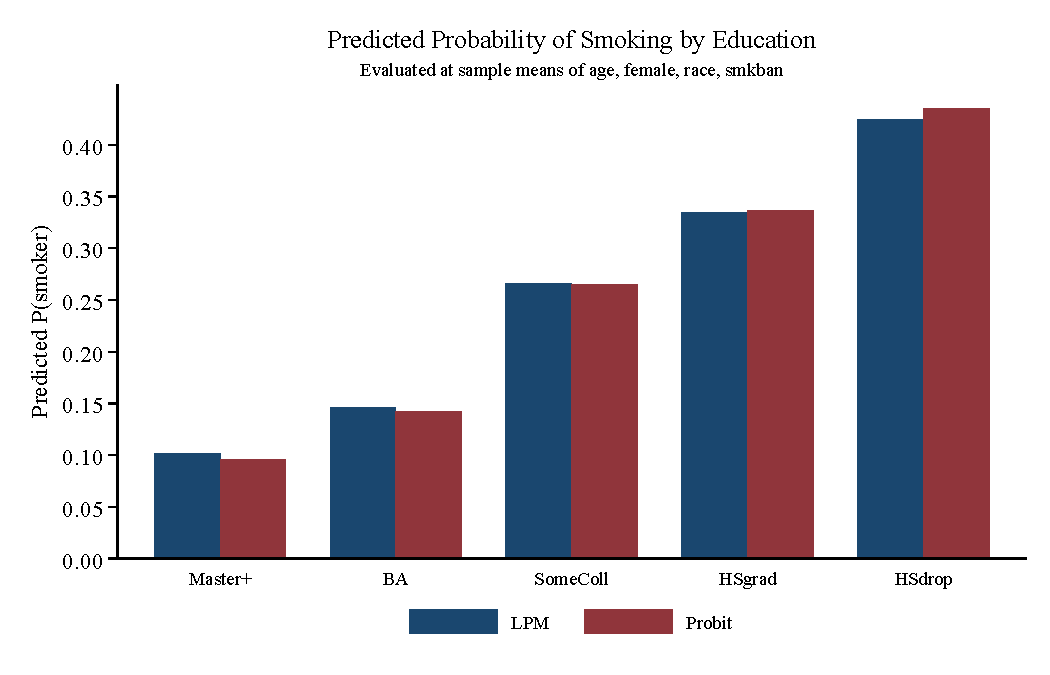
\includegraphics[width=0.92\textwidth]{output/figures/prob2_predprob_educ.pdf}
\caption{Predicted probability of smoking by education category, holding all other covariates at their sample means. LPM and probit yield indistinguishable predictions. The probability of smoking is monotonically decreasing in education. Source: own calculations using \texttt{smoking.dta}.}
\label{fig:p2_educ}
\end{figure}

\newpage

\section*{Replication Files}
\addcontentsline{toc}{section}{Replication Files}

All replication materials for \texttt{homework\_06} are available on GitHub:

\begin{itemize}
    \item Course repository: \url{https://github.com/tylersotomayor/econun3412-spring2026}
    \item Homework 06 folder: \url{https://github.com/tylersotomayor/econun3412-spring2026/tree/main/homework_06}
\end{itemize}

The \texttt{do\_files/} subfolder contains \texttt{ps6\_problem1.do} (solving SW~11.1) and \texttt{ps6\_problem2.do} (solving SW~11.2), each heavily annotated with comments explaining every step of the code and output. The \texttt{output/} subfolder contains the \LaTeX\ tables (\texttt{output/tables/}) and academic-quality PDF figures (\texttt{output/figures/}) generated by those do-files and \texttt{\textbackslash input}ed into this document.

\newpage
\bibliographystyle{apalike}
\bibliography{references}

\end{document}
